%Texlive-full Version 3.141592-1.40.3 (Web2C 7.5.6)
%Kile Version 2.0.83

%File associated : Mas_Logo.ps , uncertainty.bib

\documentclass[a4paper,10pt]{article}
\usepackage[utf8x]{inputenc}

\usepackage{lmodern}
\usepackage[a4paper]{geometry}
%\usepackage[frenchb]{babel}
\usepackage{graphicx}
\usepackage{hyperref}

\usepackage{pstricks}
\usepackage{pst-node}
%\usepackage{wrapfig}
\usepackage{amsmath}
\usepackage{amssymb}
\usepackage{hyperref}
\usepackage{listings}

\begin{document}

\begin{center}
Colossus's Algorithm Test 
\end{center}
The project was done with two days of works. I develop with rigorous test in order to handle the good quality of the code. First implementation, I took a quick look to algorithms, and think more about the design. The idea is to follow agile method, develop the first version of code that works, with a good design, the algorithm should be studied and improuved easily in the second stage. 
\section{Design} 
A ideal abstract design of processing streaming data should be as the UML figure \ref{fig:uml}
\begin {figure}[h]
\begin{center}
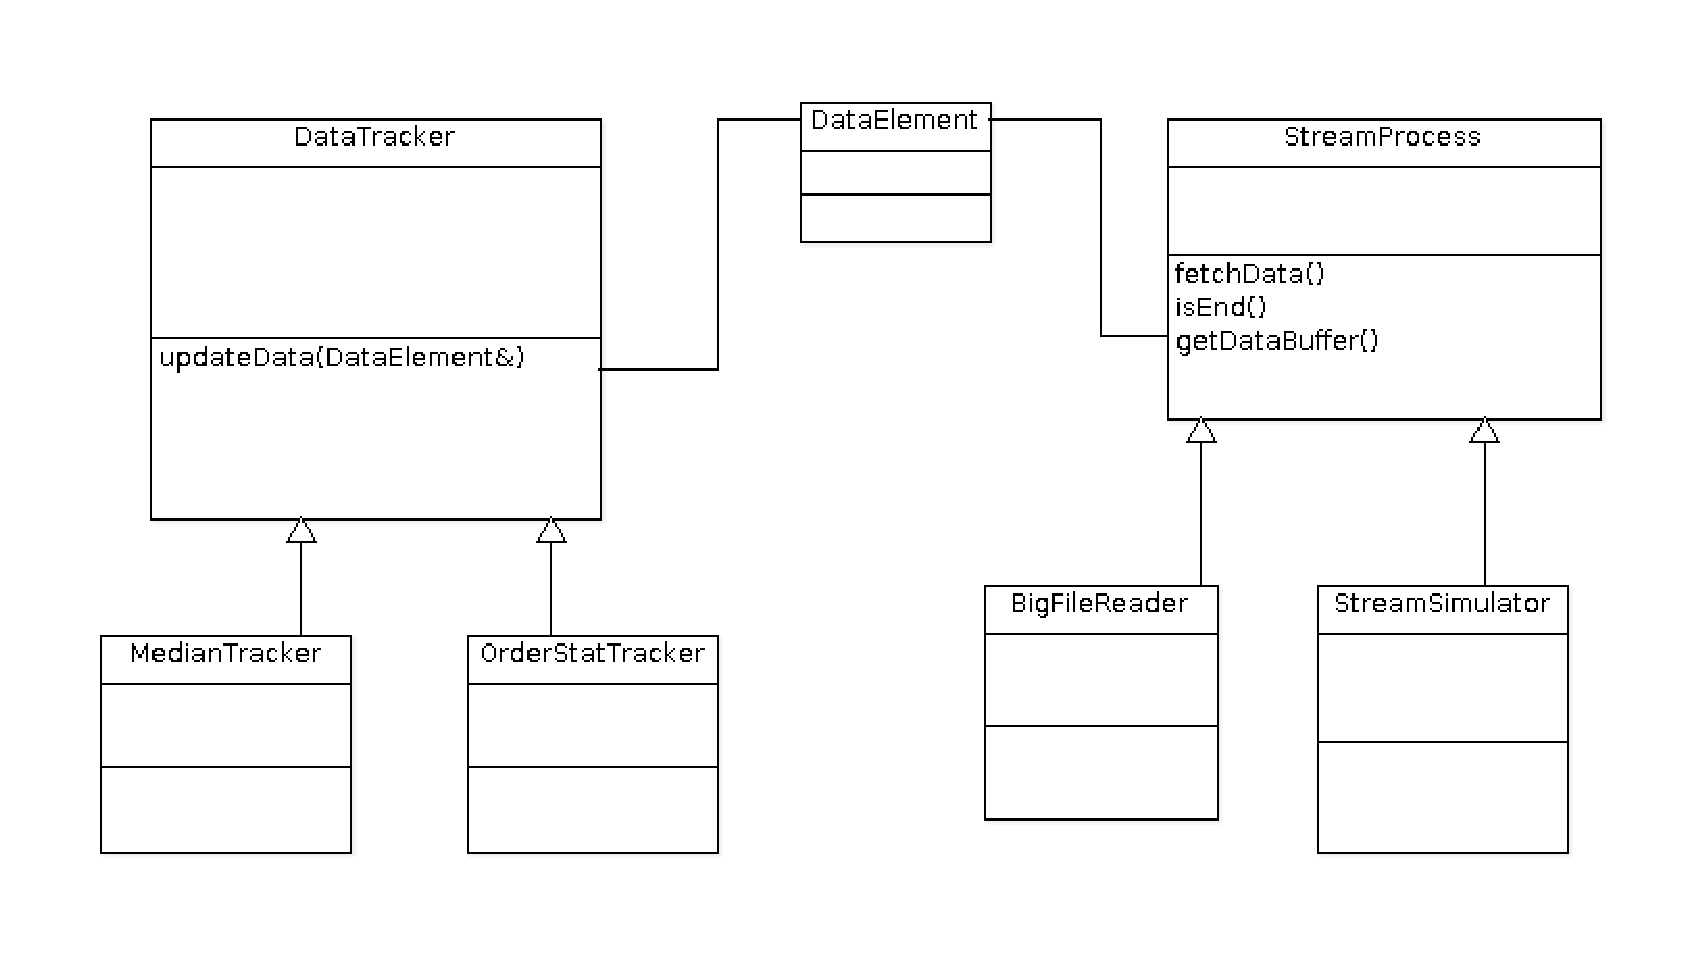
\includegraphics[scale=0.4]{ClassDiagram}
\caption{\label{fig:uml}UML}
\end{center}
\end {figure}
These module articulate around three base classes \textit{DataElement}, \textit{StreamProcess} and \textit{DataTracker}. \textit{StreamProcess} is an abstract tool who fetch the data from network, from text file, or others. One fetch will update a data buffer, which is a \textit{DataElement}, and the \textit{DataTracker} tracks the stream's properties by updating the fetched buffer. Note that when processing the stream with very small \textit{DataElement}, the call of \textit{virtual method} a billion of times should cost the performance. To avoid that, we can use the template and static polymorphic. \textit{StreamProcess} and \textit{DataTracker} should be templated on \textit{DataElement}. And their inheritances would be implemented using the \href{http://en.wikipedia.org/wiki/Curiously_recurring_template_pattern}{CTRP} pattern.      
\paragraph{} In my implementation, everythings is not already done. For the moment, the \textit{DataElement} simply is a std::vector. The \textit{Median} and \textit{Selection} classes are \textit{DataTracker} who resolve the problems of finding median and finding the k-order statistic. The base class \textit{DataTracker} did not exist but can be implemented easily. I also implement two \textit{StreamProcess}, one is a simulator that simulate data, the other read the stream from a text file. The existence of simulator allow ease for tests.

\section{Algorithms}
The very trivial algorithm idea is to fetch data from the stream, store everying in a whole container, and do the sort for each iterations. The k-order statistic and median can hit at $\Theta(1)$ afterward. However the sort iteratively can take $\Theta(N^2)$. I took a quick look at ~\cite{THOMAS} and on internet, in particular I found that ~\cite{STACKOVERFLOW} should be reasonable for a first implementation. 
\section{k-th order statistic}
My implementation of this algorithm is to use a memory of size $k$, and slice through the stream. This method has linear complexity $\Theta(N)$, with the hidden constant inside depend of $k$. Since it depends strongly to $k$, this method suffer when $k$ is big.
\section{median}
From ~\cite{STACKOVERFLOW}, I use the min-max Heap from STL for tracking the median. First implementation works and is tested correctly. For the moment, I am aware that it is not an optimal method, but if there are a litle more time, this should be improved quickly with the flexible design. The big downside of this method is the median's tracker has to store the whole container. The push operator into the heap take $\Theta(\text{log}n)$, by iterating $N$ time through the stream, the order of complexity is about $\Theta(N\text{log}N)$. In the case of storing the whole data, Thomas ~\cite{THOMAS} can give an algorithm in linear time, but a bit more complicated to implement. 
\paragraph{} The fact that one want the exact median need to store the whole data stream. If only an approximation is required, the constraint of storing-whole-data can be relaxed, but one need to study seriously how accurate the solution is. An example can look in  ~\cite{PETER1990}. 

\begin {figure}
\begin{center}
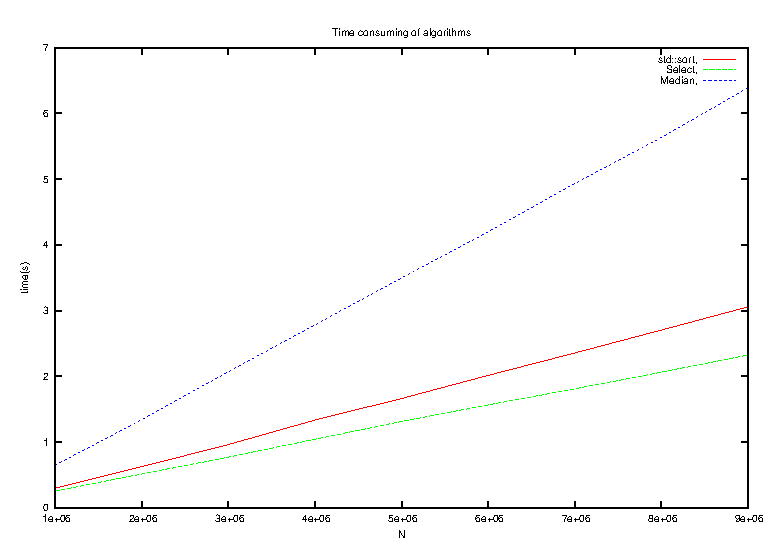
\includegraphics[scale=1.0]{output_time_measure}
\caption{\label{fig:time_measure}Time Measure of Algorithm}
\end{center}
\end {figure}
\section{Test}
Test was done rigorously. Every implementation are tested. The easiest way to test accuracy of these algorithms, is to compare the result with a full-stored-and-sorted container. The tests was run many times, with random input : each time the simulator give a different input, that make tests more credible.
\paragraph{} A test was also done in order to measure the time of these algorithm, and compare them. Three algorithms turns with different size of data (the whole data with size $N$)
\begin{itemize}
 \item std::sort
 \item find median
 \item find 10-order statistic
\end{itemize}
Results are printed in \ref{fig:time_measure}. The good point is all the three algorithms are nearly linear. However the algorithms of sorting from STL and finding median that I implement are supposed to have the complexity $\Theta(N\text{log}N)$. The fact that they are nearly linear require more studies on the time comsuming of these algorithms.
\bibliographystyle{siam}
\bibliography{OnlineSelection}
\end{document}